% Options for packages loaded elsewhere
\PassOptionsToPackage{unicode}{hyperref}
\PassOptionsToPackage{hyphens}{url}
%
\documentclass[
  12pt,
]{article}
\usepackage{amsmath,amssymb}
\usepackage{lmodern}
\usepackage{iftex}
\ifPDFTeX
  \usepackage[T1]{fontenc}
  \usepackage[utf8]{inputenc}
  \usepackage{textcomp} % provide euro and other symbols
\else % if luatex or xetex
  \usepackage{unicode-math}
  \defaultfontfeatures{Scale=MatchLowercase}
  \defaultfontfeatures[\rmfamily]{Ligatures=TeX,Scale=1}
\fi
% Use upquote if available, for straight quotes in verbatim environments
\IfFileExists{upquote.sty}{\usepackage{upquote}}{}
\IfFileExists{microtype.sty}{% use microtype if available
  \usepackage[]{microtype}
  \UseMicrotypeSet[protrusion]{basicmath} % disable protrusion for tt fonts
}{}
\makeatletter
\@ifundefined{KOMAClassName}{% if non-KOMA class
  \IfFileExists{parskip.sty}{%
    \usepackage{parskip}
  }{% else
    \setlength{\parindent}{0pt}
    \setlength{\parskip}{6pt plus 2pt minus 1pt}}
}{% if KOMA class
  \KOMAoptions{parskip=half}}
\makeatother
\usepackage{xcolor}
\usepackage[margin=1in]{geometry}
\usepackage{graphicx}
\makeatletter
\def\maxwidth{\ifdim\Gin@nat@width>\linewidth\linewidth\else\Gin@nat@width\fi}
\def\maxheight{\ifdim\Gin@nat@height>\textheight\textheight\else\Gin@nat@height\fi}
\makeatother
% Scale images if necessary, so that they will not overflow the page
% margins by default, and it is still possible to overwrite the defaults
% using explicit options in \includegraphics[width, height, ...]{}
\setkeys{Gin}{width=\maxwidth,height=\maxheight,keepaspectratio}
% Set default figure placement to htbp
\makeatletter
\def\fps@figure{htbp}
\makeatother
\setlength{\emergencystretch}{3em} % prevent overfull lines
\providecommand{\tightlist}{%
  \setlength{\itemsep}{0pt}\setlength{\parskip}{0pt}}
\setcounter{secnumdepth}{-\maxdimen} % remove section numbering
\usepackage{fancyhdr}
\usepackage{fontspec}
\usepackage{xcolor}
\usepackage{hyperref}
\usepackage{pdfcomment}

\setmainfont{Poppins}

\fancypagestyle{plain}{\pagestyle{fancy}} % added to show header and footer in the first page

% header and footer
\pagestyle{fancy}
\setlength{\headheight}{75pt}
\setlength{\textheight}{600pt}
\fancyhead[C]{}
\fancyhead[L]{\includegraphics{X:/DSA/shiny-uploads/images/trends-header.png}}
\fancyhead[R]{}
\newdateformat{monthyeardate}{\monthname[\THEMONTH] \THEYEAR}
\fancyfoot[L]{\scriptsize{1011 Western Ave, Suite 500, Seattle WA 98104} \textcolor[HTML]{F05A28}. 206.464.7532 \textcolor[HTML]{F05A28}. www.psrc.org \textcolor[HTML]{F05A28}. \monthyeardate\today}
\fancyfoot[R]{\textcolor[HTML]{F05A28}\thepage}
\fancyfoot[C]{}
\renewcommand{\headrulewidth}{0pt}
\renewcommand{\footrulewidth}{4pt}
\renewcommand{\footrule}{\hbox to \headwidth{\color[HTML]{BCBEC0}\leaders\hrule height \footrulewidth\hfill}}
\ifLuaTeX
  \usepackage{selnolig}  % disable illegal ligatures
\fi
\IfFileExists{bookmark.sty}{\usepackage{bookmark}}{\usepackage{hyperref}}
\IfFileExists{xurl.sty}{\usepackage{xurl}}{} % add URL line breaks if available
\urlstyle{same} % disable monospaced font for URLs
\hypersetup{
  hidelinks,
  pdfcreator={LaTeX via pandoc}}

\author{}
\date{\vspace{-2.5em}}

\begin{document}

\hypertarget{trends-in-employment-and-telecommuting}{%
\section{Trends in Employment and
Telecommuting}\label{trends-in-employment-and-telecommuting}}

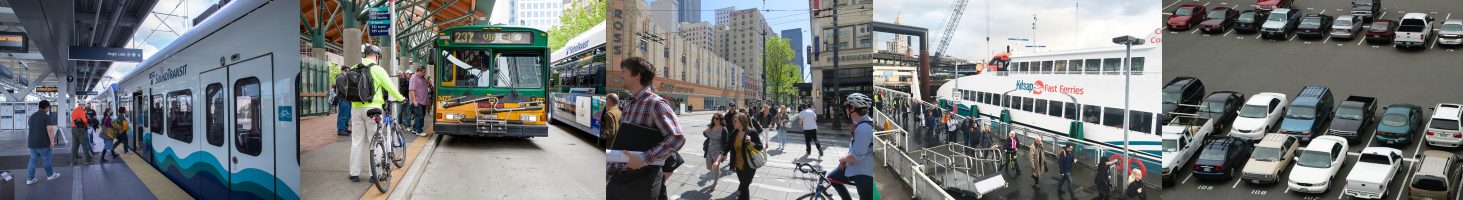
\includegraphics[width=1\textwidth,height=\textheight]{X:/DSA/Trends/household-travel-survey/images/employment_telecommuting_header.png}

\begin{flushleft}
The 2021 regional travel survey collected day-to-day information from households in the central Puget Sound region: how we traveled, where we went, how long it took - even where we chose to live and whether we got home deliveries. This report compares household travel choices in 2021, during COVID-19 conditions to that in the previous years of 2017 and 2019. In some analysis 2017 and 2019 survey samples have been combined to strengthen the statistical validity of the findings by increasing the number of respondents included in the analysis. Learn more at the \href{https://www.psrc.org/our-work/household-travel-survey-program}{\underline{\textcolor{blue}{PSRC household travel survey webpage}}}. You can also \href{https://household-travel-survey-psregcncl.hub.arcgis.com}{\underline{\textcolor{blue}{view the full travel survey dataset here}}}, including 2017, 2019, and 2021 data.
\end{flushleft}

\hypertarget{major-workplace-changes-happened-in-2021}{%
\subsection{Major workplace changes happened in
2021}\label{major-workplace-changes-happened-in-2021}}

\begin{flushleft}
In the regional travel surveys from 2017 to 2021, respondents with jobs were asked to select their current work location from a list of options. In the 2017/2019 combined survey, people  who from home comprised only 6\% of all workers in the region. By spring of 2021, the portion of people working from home increased dramatically to 27\% of all workers in the region. Combined with the portion of people that teleworked some days and traveled to work some days, we saw 37\% of workers in the region working from home at least part of the time. However, the majority of workers in 2021 still traveled to a work location outside of the home.
\end{flushleft}

\begin{center}\includegraphics{telecommute_2021_mr_files/figure-latex/workplace-1} \end{center}

\hypertarget{large-changes-seen-in-telecommuting}{%
\subsection{Large changes seen in
telecommuting}\label{large-changes-seen-in-telecommuting}}

\begin{flushleft}
Working remotely from home, also called telecommuting, has been a feature of the work environment in the Puget Sound region for multiple years before the onset of the COVID-19 pandemic. While it is true that the pandemic lead to major increase in telecommuting, we saw that a trend was already underway in the two travel surveys before 2021.
\end{flushleft}

\hypertarget{yearly-increases-in-weekly-rates-of-telecommuting}{%
\subsubsection{Yearly increases in weekly rates of
telecommuting}\label{yearly-increases-in-weekly-rates-of-telecommuting}}

\begin{flushleft}
In the travel surveys, people who responded that they traveled to a primary work location or, in 2021, telecommuted some days and traveled to work some days were asked to state how often they had substituted a work trip with telecommuting in the past week. In 2017, 16\% of those workers telecommuted at least once per week; this increased slightly to 20\% in 2019, followed by a large increase to 31\% in 2021.
\end{flushleft}

\begin{center}\includegraphics{telecommute_2021_mr_files/figure-latex/telecommute_over_year-1} \end{center}

\hypertarget{telecommute-frequencies-did-not-increase-evenly}{%
\subsubsection{Telecommute frequencies did not increase
evenly}\label{telecommute-frequencies-did-not-increase-evenly}}

\begin{flushleft}
When looking at a more detailed view of telecommuting frequency, the largest increase occurred for workers who said they telecommuted 3-4 days per week, increasing from around 2\% in 2017 to 10\% in 2021. Telecommuting five or more days per week also saw a large increase, while telecommuting only one or two times per week did not increase after 2019.
\end{flushleft}

\begin{center}\includegraphics{telecommute_2021_mr_files/figure-latex/times_per_week-1} \end{center}

\hypertarget{telecommute-frequency-varied-by-gender}{%
\subsubsection{Telecommute frequency varied by
gender}\label{telecommute-frequency-varied-by-gender}}

\begin{flushleft}
When telecommute frequency is broken down by gender, there was little difference in the shares of female workers reporting telecommuting 1-2 days per week (11\%), 3-4 days per week (12\%), and 5+ days per week (10\%). There was a slightly larger difference for male workers, with the largest share reporting 5+ days per week (12\%) compared to 9\% and 8\% for 1-2 days per week and 3-4 days per week, respectively. For both genders, the largest increase in telecommuting frequency between 2017/2019 and 2021 was for 3-4 days per week; the share of female workers increased from 2\% to 12\% and the share of male workers increased from 3\% to 8\%. There was also a large increase in male workers who reported telecommuting 5+ days per week, an increase from 7\% to 12\%.
\end{flushleft}

\begin{center}\includegraphics{telecommute_2021_mr_files/figure-latex/telecommute_gender-1} \end{center}

\hypertarget{telecommute-frequency-also-varied-by-race-and-ethnicity}{%
\subsubsection{Telecommute frequency also varied by race and
ethnicity}\label{telecommute-frequency-also-varied-by-race-and-ethnicity}}

\begin{flushleft}
When telecommute frequency is broken down by race and ethnicity, the number of workers telecommuting at least once per week increased the most for white workers, while telecommuting remained the same for workers of color. By the 2021, there were similar shares of workers of color and white workers telecommuting.

**SHOULD WE INCLUDE A GRAPH HERE SHOWING THIS TREND?**

\end{flushleft}

\hypertarget{trends-in-workplace-travel-and-worker-industry-in-2021}{%
\subsection{Trends in workplace travel and worker industry in
2021}\label{trends-in-workplace-travel-and-worker-industry-in-2021}}

\begin{flushleft}
As discussed above, 37\% of workers in the region worked at home in 2021, while 63\% of workers still worked at a location outside the home. However, we did see differences in the survey data when cross-tabulating differences in workplace travel by gender and by race and ethnicity.
\end{flushleft}

\hypertarget{males-working-outside-the-home-more-than-females}{%
\subsubsection{Males working outside the home more than
females}\label{males-working-outside-the-home-more-than-females}}

\begin{flushleft}
Overall, there was a greater proportion of male workers (66\%) who reported working outside the home than female workers (59\%). However, both groups deviate only slightly from the regional average of 63\% of workers.
\end{flushleft}

\hypertarget{more-african-american-and-hispanic-workers-working-outside-the-home}{%
\subsubsection{More African American and Hispanic workers working
outside the
home}\label{more-african-american-and-hispanic-workers-working-outside-the-home}}

\begin{flushleft}
When broken down by race and ethnicity, a greater proportion of African American (71\%) and Hispanic (78\%) workers reported working outside the home than the regional average.
\end{flushleft}

\hypertarget{differences-seen-in-workplace-travel-based-on-worker-industry}{%
\subsubsection{Differences seen in workplace travel based on worker
industry}\label{differences-seen-in-workplace-travel-based-on-worker-industry}}

\begin{flushleft}
PSRC first began asking survey respondents in which industry they worked in the 2021 household travel survey. We used industry groups to see differences in workplace travel based on workers' fields of employment. We found that there were five industry groups with workers reporting that they worked outside the home more than the regional average (63\%; green bar in chart below): Military (98\%); Personal Services (85\%); Hospitality \& Retail (81\%); Health Care, Social Services \& Childcare (81\%); and Construction \& Resources (79\%).
\end{flushleft}

\begin{center}\includegraphics{telecommute_2021_mr_files/figure-latex/industry_work_travel-1} \end{center}

\begin{flushleft}
Of those five industry groups that worked outside the home more than the regional average, two had greater proportions of female workers than the regional average (45\%; green bar in chart below): Health Care, Social Services \& Childcare (73\%) and Personal Services (69\%).

**MORE DETAIL ABOUT THE REMAINING BREAKDOWN FOR THE OTHER THREE**

\end{flushleft}

\begin{center}\includegraphics{telecommute_2021_mr_files/figure-latex/industry_gender-1} \end{center}

\begin{flushleft}
Of those five industry groups that worked outside the home more than the regional average, three had greater proportions of workers of color than the regional average (33\%; green bar in chart below): Health Care, Social Services \& Childcare (42\%); Hospitality \& Retail (41\%); and Personal Services (39\%).

**CHART NUMBERS STILL OFF?**

\end{flushleft}

\begin{center}\includegraphics{telecommute_2021_mr_files/figure-latex/industry_race-1} \end{center}

\subsection{Conclusion}
\begin{flushleft}

conclusion text here

\end{flushleft}

\end{document}
